%%This is a very basic article template.
%%There is just one section and two subsections.
\documentclass{article}
\usepackage[a4paper, margin=2.5cm]{geometry}
\usepackage{amsmath}
\usepackage{caption}
\usepackage{placeins}
\usepackage{graphicx}
\usepackage{subcaption}
\usepackage{setspace}
\usepackage{float}
\usepackage{wrapfig}
\usepackage{pdfpages}
%\usepackage[active,tightpage]{preview}
\usepackage{natbib}
\bibpunct{(}{)}{,}{a}{}{;} 
\usepackage{url}
\usepackage{nth}
\usepackage{authblk}
\usepackage{blindtext}
% for the d in integrals
\newcommand{\dd}{\; \mathrm{d}}
\newcommand{\tc}{\quad\quad\text{,}}
\newcommand{\tp}{\quad\quad\text{.}}
\newcommand{\ra}{\rightarrow}
\def\lsub#1#2%
  {\mathop{}%
   \mathopen{\vphantom{#2}}_{#1}%
   \kern-\scriptspace%
   #2}
\def\lsup#1#2%
  {\mathop{}%
   \mathopen{\vphantom{#2}}^{#1}%
   \kern-\scriptspace%
   #2}

\defcitealias{HMD}{HMD}
\defcitealias{HFD}{HFD}
\newcommand\ackn[1]{%
  \begingroup
  \renewcommand\thefootnote{}\footnote{#1}%
  \addtocounter{footnote}{-1}%
  \endgroup
}
\begin{document}

%\title{Macro patterns in the shape of aging}
\title{Boom, echo, pulse, flow}
\author[1]{Tim Riffe\thanks{riffe@demogr.mpg.de}}
\author[1]{Kieron Barclay}
\affil[1]{Max Planck Institute for Demographic Research}
\maketitle

\begin{abstract}
Human population renewal starts with births. Since births can happen at any
time in the year and over a wide range of ages, demographers typically imagine
the birth series as a continuous flow. Taking this construct literally, we
visualize the birth series as a flow. A long birth series allows us to
juxtapose the children born in a particular year with the children that
they in turn had over the course of their lives, yielding a crude notion of
cohort replacement. Macro patterns in generational growth define the meandering
path of the flow, while temporal booms and busts echo through the flow with the
regularity of a pulse.
\end{abstract}

\onehalfspacing
\section{Introduction}
Usually we think of fertiltiy as an age-regulated process. In any case it is
bounded by menarche and menopause, both of which are anchored to age. These anchors may
move, but not far or fast. And between these bounds, at least within acceptably homogenous subpopulations, fertility patterns appear to
conform to some regular schema, best captured by fertility rates. In this treatment, we retreat
from rates, the material of projections, to babies, the raw material of
population renewal. We use birth count data from the \citet{HFD} for Sweden, covering a total of 241 ocurrence years. These data include preliminary data for the period 1775 to 1890, which we have graduated and adjusted. We describe those steps in Appendix~\ref{sec:dataprep}. A picture of the births in a year is for demographers most
instinctively broken down by the age of mothers who gave birth in that year,
Fig.~\ref{fig:agemother}, or by the year of birth of mothers Fig.~\ref{fig:cohmother}. These two distributions are essentially identical, but appear as mirror images if chronological time is enforced in $x$.

\begin{figure}[ht!]
\begin{subfigure}[t]{0.5\textwidth}
        \centering
        \includegraphics[width=\textwidth]{Figures/Fig11900MotherAge.pdf}
        \caption{Births in 1900 by age of mother}
        \label{fig:agemother}
\end{subfigure}
~
\begin{subfigure}[t]{0.5\textwidth}
        \centering
        \includegraphics[width=\textwidth]{Figures/Fig11900MotherCohort.pdf}
        \caption{Births in 1900 by year of birth of mother}
          \label{fig:cohmother}
\end{subfigure}
\caption{Births in a year structured by mothers' age versus mothers' year of birth are a
reflection over $y$ and shift over $x$.}
\end{figure}

If one disposes of a long-enough time series of births classified by mothers' year of birth, then one may further examine and break down the full reproductive career of the cohort of individuals born in a particular year. Since the childbearing of a cohort is spread over a synchronous span of ages and years, the classification by age (Fig.~\ref{fig:age1900mother}) or year (Fig.~\ref{fig:year1900}) yields identical and redundant distributions.

\begin{figure}[ht!]
\begin{subfigure}[t]{0.5\textwidth}
        \centering
        \includegraphics[width=\textwidth]{Figures/Fig11900IDAge.pdf}
        \caption{Births from mothers born in 1900 by age of mother}
        \label{fig:age1900mother}
\end{subfigure}
~
\begin{subfigure}[t]{0.5\textwidth}
        \centering
        \includegraphics[width=\textwidth]{Figures/Fig11900IDYear.pdf}
        \caption{Births from mothers born in 1900 by year}
          \label{fig:year1900}
\end{subfigure}
\caption{Births of a cohort structured by mothers' age versus mothers' year of birth are a
reflection over $y$ and shift over $x$.}
\end{figure}

The births in a year are classified by mothers' cohort, i.e. cohort \emph{origins} in Fig.~\ref{fig:cohmother}, whereas the births \emph{from} a cohort are classified \emph{to} time in Fig.~\ref{fig:year1900}. The two distributions are different in kind, but relatable and both on a common scale. A fuller representation of their relationship would place them as two disjoint distributions on the same timeline, as in Fig~\ref{fig:juxt}.

\begin{figure}[ht!]
 \centering
        \includegraphics[width=\textwidth]{Figures/Fig31900juxt.pdf}
        \caption{Births from mothers born in 1900 by year}
          \label{fig:juxt}
\end{figure}

The two distributions in Fig.~\ref{fig:juxt} are related, and of comparable scale, but different in kind. The $x$ coordinate of the left distribution is indexed to mothers's birth cohort, whereas the $x$ coordinate of the right distribution is indexed to child cohort, ocurrence year. In this way the $x$ coordinates belong to grandmothers and grandchildren, where the \emph{ego} generation is 1900. These are two quantities that we may wish to compare in various ways to get a better feel and understanding of the Swedish birth series. 

For the case of these Swedish data, we have 241 such distribution pairs, making single-axis rendering impractical. An honest attempt might look like Fig.~\ref{fig:reflect1}, where we reflect the Fig.~\ref{fig:juxt} left distribution over $y$ (\textbf{A}), keeping the Fig.~\ref{fig:juxt} right-side distribution on top (\textbf{B}). These two distributions are linked by the year 1900, which of course overlaps with neither of them. In this representation, \textbf{A} and \textbf{B} are re-drawn for each possible ego year (1775-2015), and therefore imply a large sequential set of overlapping distributions. Each \nth{20} distribution is highlighted, but despite attempts to make this graph legible, i) the high degree of overlapping and ii) the spatial dissociation of each \textbf{A} --- \textbf{B} pair makes the intended comparison difficult over the series.

\begin{figure}[ht!]
 \centering
        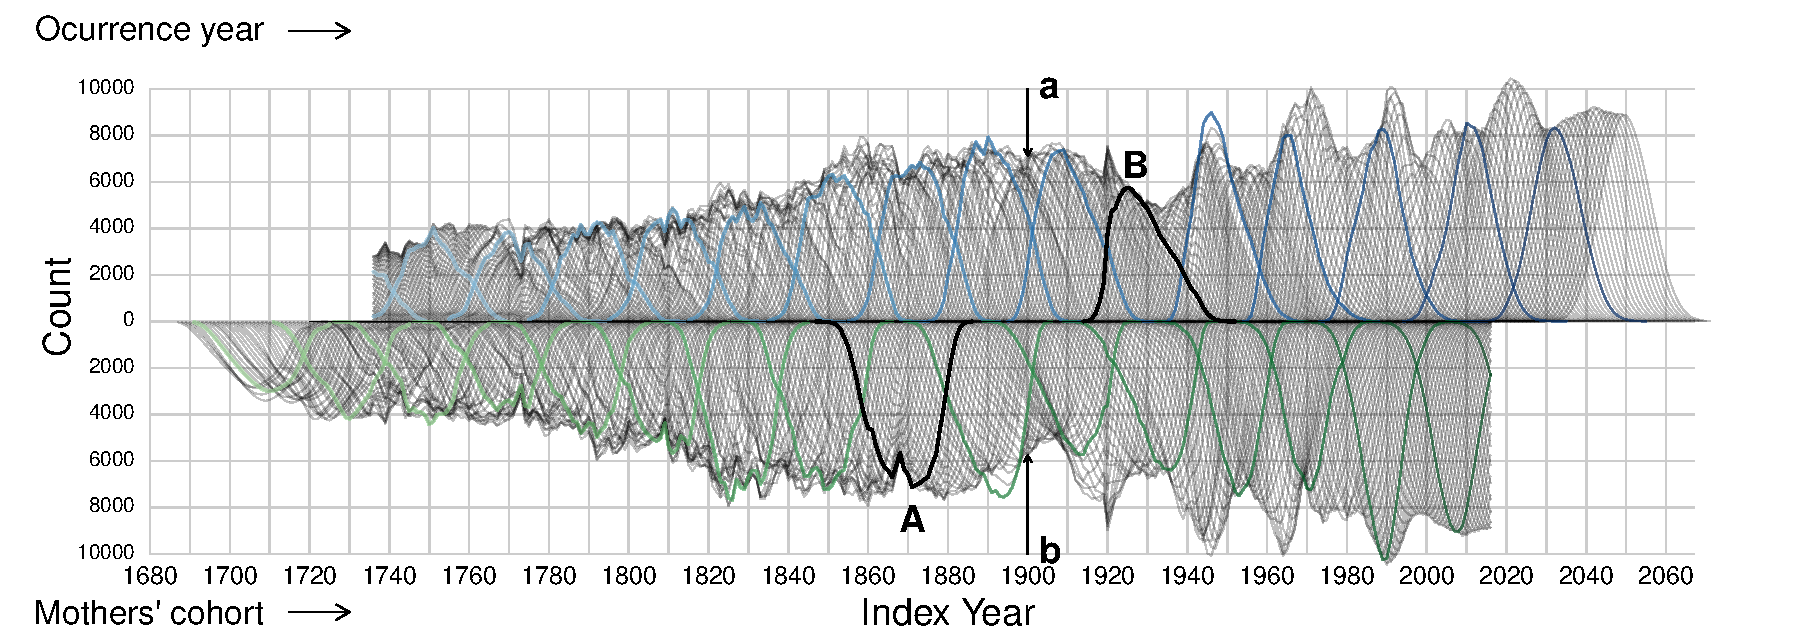
\includegraphics[width=\textwidth]{Figures/FxFlowReflect.pdf}
        \caption{Two time series of birth count distributions. The top series is composed of offspring distributions of mother cohorts over time, indexed to ocurrence years. The bottom series is composed of the offspring of a year indexed to mothers' birth cohorts. \textbf{B} is the offspring of mothers from the 1900 cohort indexed in $x$ to ocurrence year, and \textbf{A} are the births ocurred in 1900 indexed in $x$ to mothers' birth cohorts. The cross-section \textbf{a} gives \textbf{A} and the cross-section \textbf{b} gives \textbf{B}.}
          \label{fig:reflect1}
\end{figure}

Fig.~\ref{fig:reflect1} produces at least two noteworthy artifacts that we may wish to preserve or clarify. 1) First order differences in the top series appear to cascade into the lower series--- This merely points out that larger cohorts have more offspring than smaller neighboring cohorts and vice versa, sudden fertility rate changes notwithstanding. 2) The composition of \textbf{A} in the bottom series is implied by the cross-section \textbf{a} of the top series, and the composition of  \textbf{B} is implied by the cross-section \textbf{b}. To reiterate: \textbf{A} are all the births in 1900 indexed back to mothers' cohorts. Each possible \emph{slice} of \textbf{A} comes from a different top distribution as it crosses the year 1900 (and vice versa for the bottom). \textbf{a} and \textbf{b} are in a sense already juxtaposed for us, as they share an $x$ coordinate. The ``problem'' with the cross-sections \textbf{a} (\textbf{b}) is that each \emph{slice} of the corrsponding distribution \textbf{A} (\textbf{B}) is perfectly overlapped, such that it is just about impossible to imagine what \textbf{A} might look like if presented only with \textbf{a} and its surroundings. 
% Q: should the 'pointers' for a and b actually be drawn on top of the data series, as of a cross-section?
\pagebreak
% text above pushes whole thing down
\begin{wrapfigure}{r}{0.5\textwidth}
 \centering
        \includegraphics[width=3in]{Figures/FigReflection.pdf}
        \caption{The 1900 cohort as a composite bar with its offspring reflected over $y$. The size of each bar stacked in the top composition is proportionate to the area of its corresponding polygon in the left distribution of Fig.~\ref{fig:juxt}. The size of each bar stacked in the lower composition is proportionate to the area of its corresponding polygon in the right distribution of Fig.~\ref{fig:juxt}.}
          \label{fig:refl}
\end{wrapfigure}
% text under goes to the left then builds down
In this way the two distributions that we might wish to compare for a given ego
year are already available at a like coordinate, but comparison is stifled by
overplotting. If instead we stack the slices that are indecipherably overlapped
in \textbf{a} (and likewise for \textbf{b}) we get something like that shown in
Fig.~\ref{fig:refl}, cumulative birth distributions.\footnote{Young mothers are
on top and older mothers on bottom for both distributions. It would also make
sense to plot increasing (or decreasing) ages eminating out from the centerline
in both directions.} Here the total bar length is proportional to the total
cohort (offspring) size, and stacked bins reflect 5-year mother cohorts
(ocurrence years). From this representation it is clear that mothers born in the
20 years between 1860 and 1880 produced the bulk of the 1900 cohort (86\%),
which itself produced the majority of its offspring in the 20 years between 1920
and 1940 (90\%). It is also quite visible that the 1900 cohort did not replace
itself in a crude sense: 138,139 babies formed a cohort whose mothers gave birth
to 95,379 babies over their lifecourse, a crude replacement of 69\%. Other
perspectives on reproduction that account for survival and attrition of the
mother cohort through migration would give a more optimistic assessment. The key
feature of Fig.~\ref{fig:refl} is that the two distributions that were disjoint in Fig.~\ref{fig:juxt} and hard to pick out in Fig.~\ref{fig:reflect1} can now be associated at a common $x$ coordinate. This virtue allows us to view the time series of Fig.~\ref{fig:reflect1} with greater clarity and perhaps reveal some macro properties of the history of Swedish natality.

Fig.~\ref{fig:foldout} is a depiction of the exercise of Fig.~\ref{fig:refl}, cohort bars on top reflected with offspring bars on the bottom. Equal bounded bins from Fig.~\ref{fig:refl} are joined into continuous regions. For the top region, filled polygons represent the births of mothers from quinquennial cohorts, spread over time. For the bottom region, filled polygons represent the mother-cohort origins of the births in quinquennial periods. The darkness and saturation of polygon fill colors are approximately proportional to the total births in the polygon (and therefore true to grayscale printing), whereas hue is irrelevant. In this way, darkness and saturation on the top are proportional to total height (with respect to baseline) on the bottom, and vice versa. 

The meandering baseline of Fig.~\ref{fig:foldout} is proportional to a smoothed time series of the crude cohort replacement rate. We overlay a horizontal line to indicate periods of approximate growth, replacement, and contraction. Periods where the meandering $x$-baseline is above this line (ca 1780 to 1860) indicate crude growth, and periods below the horizontal reference line (ca 1870 to 1930) indicate crude generation contraction. 

To aid the viewer with interpretation, we overlay a known lineage of five female generations,\footnote{This lineage can be located in the public domain on \url{https://www.geni.com/people/Karin-Ottolina-Landsten/6000000022470480183}.} where $x$ position is exact to the year, $y$ position in the top region is matched to the mothers cohort, and $y$ position in the bottom is matched to daughters' year of birth. Wider horizontal spacing between generations over time indicates increasing ages at maternity within this lineage (increasing from 23 to 39).

Several macro features come to the fore in this visualization. These are either known features of the Swedish birth series, or else mention further study. Echoes, booms, why is boom periodicity a recent phenomenon? Is there a dose-response to vertical reverberation in first derivative (can this be referred to as first or second order?) features.

To be continued.

\begin{figure}
\centering
[fold-out figure 125cm wide by 30cm tall at 100\% in separate pdf, about here.]
%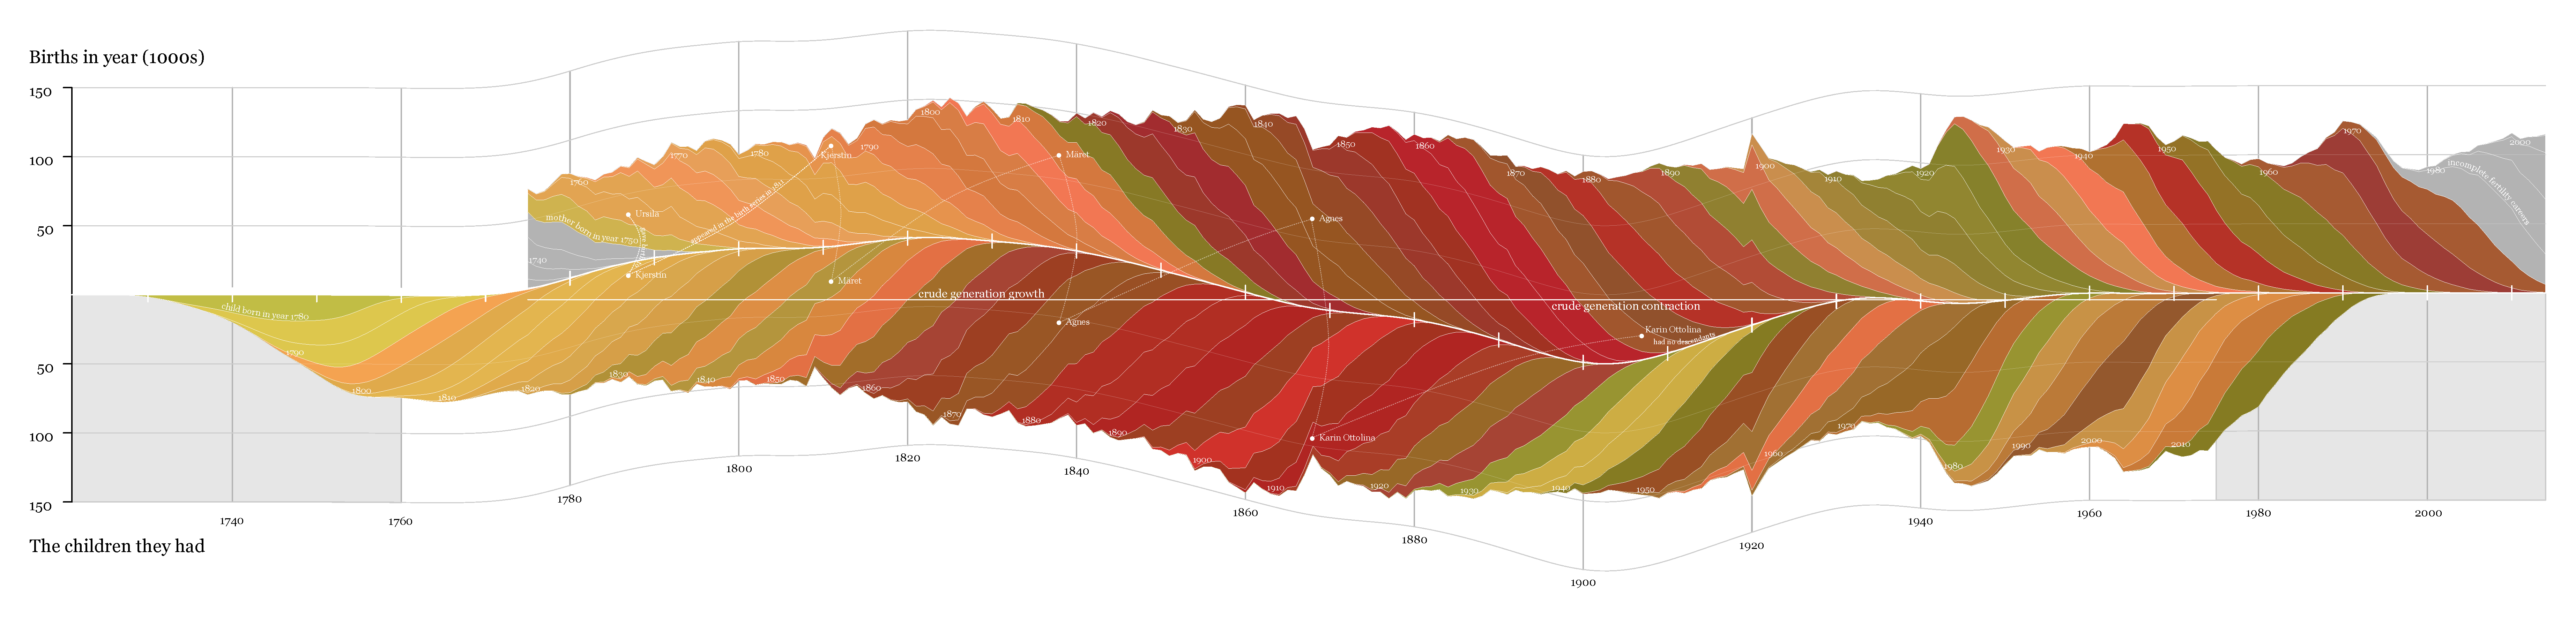
\includegraphics[scale=.9]{Figures/SwedenBirthFlowsManFoldout.pdf}
%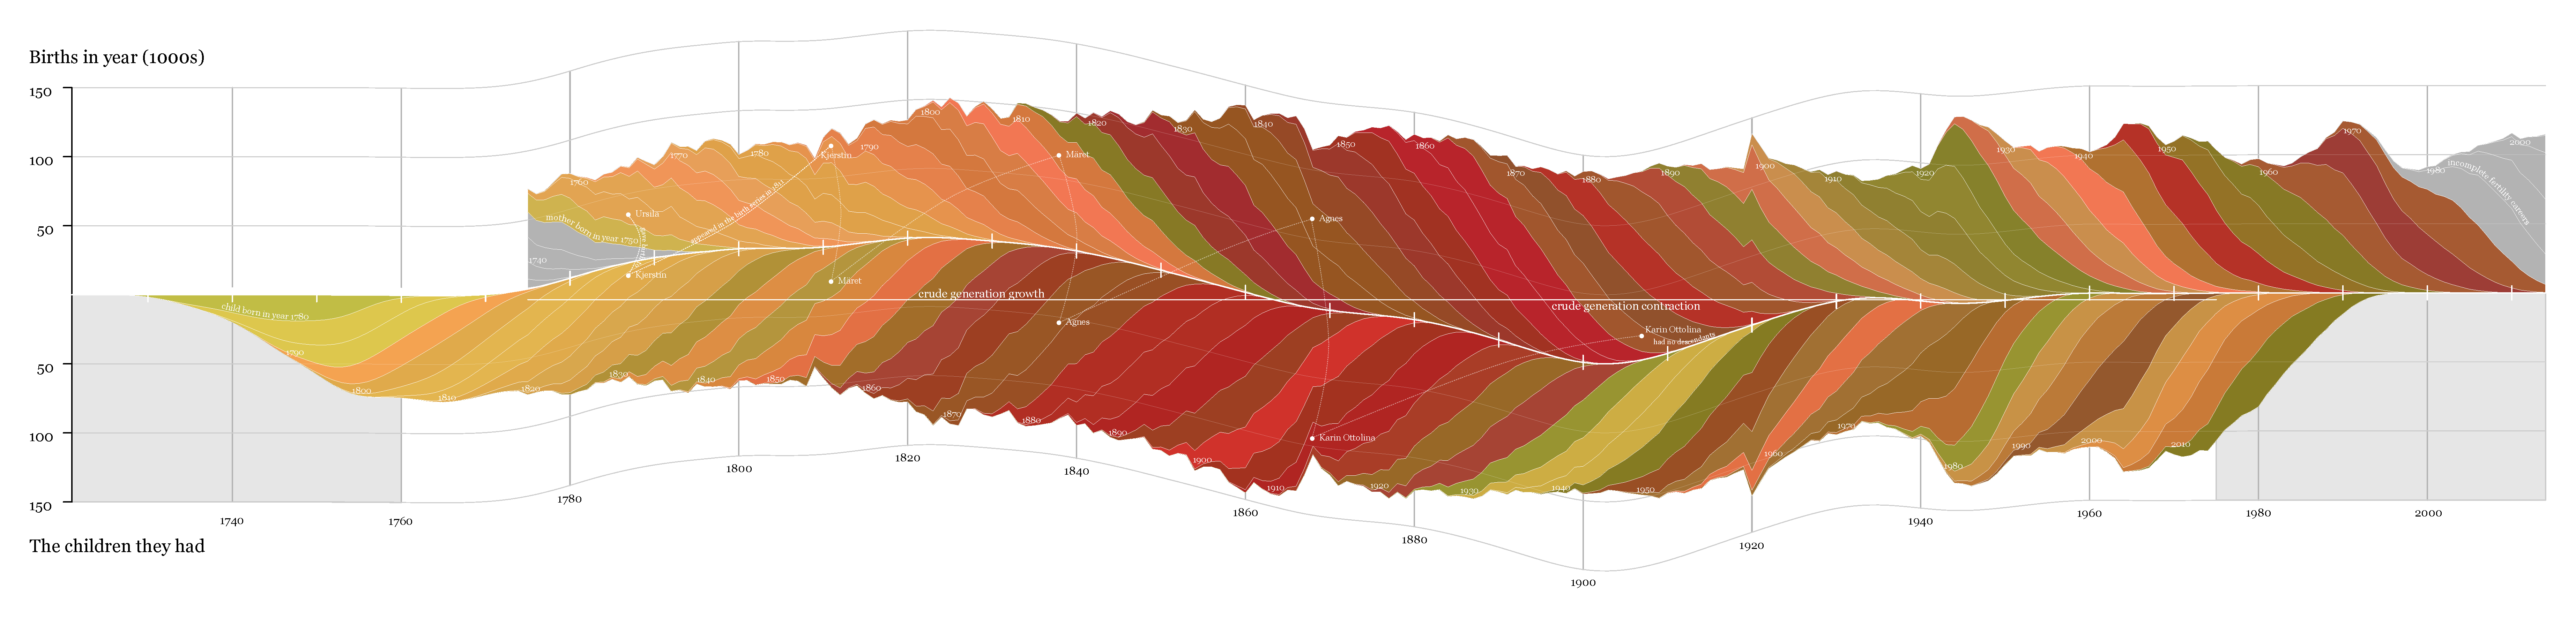
\includepdf[landscape]{Figures/SwedenBirthFlowsManFoldout.pdf}
\caption{A time series of the same graphical construct as presented in Fig.~\ref{fig:refl}. The $x$ axis now meanders proportional to a smoothed time series of the crude cohort replacement rate. Fill color darkness and saturation are approximately proportional to the total number of births in each birth distribution. The birth series now appears as a flow, but reveals echoes in cohort and offspring size, an odd periodicity in recent decades, and a long term dampening of the crude replacement rate. A 5-generation female lineage is annotated atop to serve as a guide.}
\label{fig:foldout}
\end{figure}

\begin{appendix}
\section{Data sources and adjustments}
\label{sec:dataprep}
Data presented here are from two separate files from the \citet{HFD}. The first
contains birth counts in the period-cohort Lexis shape,
\texttt{SWEbirthsVV.txt}, as produced by the HFD according to the Methods
Protocol \citep{hfd2015methods}. This file contains births by calendar year and
mother birth cohort for the years 1891 until 2015, and we use it as-is. The
second file contains births for ocurrence years 1775 until 1890. These data are
age-period classified, and given in a mixture of age classes, including a
predominance 5-year age classes (especially for ages 20-50), but also sometimes
single ages (especially for ages 15-19), and time-varying top and bottom open
ages.

It is this second file, with data covering years 1890 and earlier, that we have
adjusted in four main steps. First, births of unknown maternal age were redistributed proportionally to the distribution of births of known maternal age. Second, counts were graduated to single ages using the graduation method proposed by \citet{rizzi2015efficient} and implemented in \texttt{R} in the package \texttt{pclm}\footnote{The \texttt{pclm} package has since been extensively modified, and it is now called \texttt{ungroup} \citep{pclmR}}. Third, counts were shifted into period-cohort Lexis bins assuming that half of the births in each single age $x$ bin go to the lower triangle of age $x+1$ and half to the upper triangle of the age-reached-during-the-year (PC) parallelogram at age $x$, as diagramed in Fig.~\ref{fig:AP2PC}.

\begin{figure}
\centering
\begin{subfigure}{.3\textwidth}
  \centering
  \includegraphics[scale=.6]{Figures/App_split1.pdf}
  \caption{AP square bins}
  \label{fig:app1}
\end{subfigure}%
\begin{subfigure}{.3\textwidth}
  \centering
  \includegraphics[scale=.6]{Figures/App_split2.pdf}
  \caption{Split evenly to triangles}
  \label{fig:app2}
\end{subfigure}
\begin{subfigure}{.3\textwidth}
  \centering
  \includegraphics[scale=.6]{Figures/App_split3.pdf}
  \caption{Regroup to PC bins}
  \label{fig:app3}
\end{subfigure}
\caption{The count regrouping procedure for years 1776 to 1890, step three of data adjustment. Data are graduated to single ages (Fig.~\ref{fig:app1}), then split in half (Fig.~\ref{fig:app2}) and regrouped to period cohort (PC) bins (Fig.~\ref{fig:app3}).}
\label{fig:AP2PC}
\end{figure}
At this stage data are binned and Lexis-conformable with HFD data for years 1891 and forward. With data processed as of step three, one could produce two time series that could in principle be used to produce Fig.~\ref{fig:foldout}, with a subtle artifact visible in the following figure.

\begin{figure}
\centering
 \includegraphics[scale=.6]{Figures/App_preAdjustment.pdf}
\caption{In reference years $\ge$ 1891 both births by year and cohort offspring are directy observed in single year bins, which means that the structural echo in first differences in preserved. Births in single ocurrence years $\le$ 1890  (\textbf{A}) are presumed accurate, and so first differences of these are observd. Offspring from cohorts born before 1891 (\textbf{B}) are derived from mother cohorts (\textbf{A}) that were graduated to single ages from quinquennial ages, inducing smoothness.}
\end{figure}

\end{appendix}

\singlespacing
\bibliographystyle{plainnat}
  \bibliography{references} 
\end{document}
